\documentclass[12pt,a4paper]{article}
\usepackage[latin1]{inputenc}
\usepackage{amsmath}
\usepackage{amsfonts}
\usepackage{amssymb}
\usepackage{listings}
\usepackage{color}
\usepackage{hyperref}
\usepackage{graphicx}
\definecolor{lightGray}{gray}{0.95}
\lstset{
backgroundcolor=\color{lightGray},
breaklines=true,
captionpos=b,
frame=single,
keepspaces=true,
keywordstyle=\color{blue},
language=HTML,
morekeywords={created,modified,tags},
numbers=left
}
\title{Analysis and documentation of a single page application based on TiddlyWiki}
\author{Christian Jurke 898872, Christian Heigele 901361}
\begin{document}
\maketitle
\tableofcontents
\textbf{Pages Min:13 Max:17 }
\section{Introduction 1}
\section{Decomposition of the TiddlyWiki-Architecture 3}
\subsection{Architecture of the single page application TiddlyWiki 1}
\begin{figure}[hbtp]
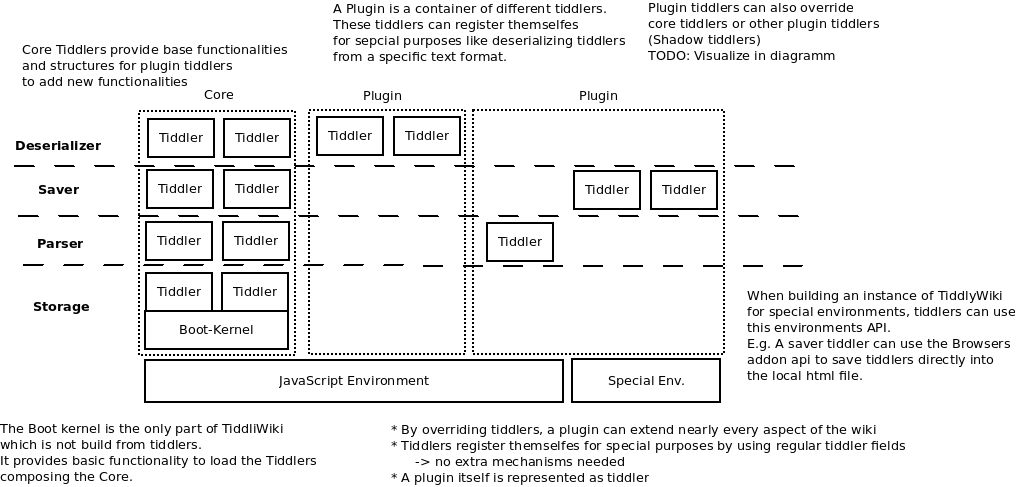
\includegraphics[scale=0.4]{images/overview.png}
\caption{Decomposition of TW}
\end{figure}

\subsection{Tiddler as the key element 1}
\subsection{The WikiText concept 1}
\section{Bootstrap-Process 2-3}
\subsection{The Heart of TiddlyWiki (Boot-Kernel) 1 - 1.5}
\subsection{Timeline of the startup Process 1 - 1.5}
\section{The Plugin and Module concept 4-5}
\subsection{Introduction to the Plugin-Concept 1}
\subsection{Kernel-Plugins 1}
\subsection{UI-Elements 1}
\subsection{Developing a own Plugin 1-2}
\section{The TiddlyWiki data management concept 2-3}
\subsection{Data Management during Runtime 1-2}
\newpage 
\subsection{Data Persistence 1}
\subsubsection*{Persist data}
TiddlyWiki supports a wide rage of methods to persist your data. One of this methods is the HTML5 fallback saver. This methods works on almost every browser. With this method a copy of the entire wiki will be downloaded by the browser. This means you get a new file everytime you hit the save button. To avoid this there a some plugins for different browsers to allow to save direct to the current open TiddlyWiki-File.
\subsubsection*{Data-Storage}
TiddlyWiki persists the data within the HTML-File in two Div-Areas depending on whether the encryption of the TiddlyWiki is activated or not. If the TiddlyWiki is not encrypted the data is stored in the Div-Area called ``StoreArea''. Every created Tiddler is stored in a own Div-area with a few custom values. An example of a saved Tiddler is shown below.
\begin{lstlisting}[caption={Data-Div}]
<div created="20140611153703343" modified="20140611153734589" tags="testTag" testfield="testvalue" title="TestTiddler" type="text/plain">
	<pre>testText</pre>
</div>
\end{lstlisting}
With a activated encryption the data is stored in a special Div-Area called ``encryptedStoreArea''. TiddlyWiki uses the Standford JavaScript Crypto Libary\footnote{\url{http://bitwiseshiftleft.github.io/sjcl/}}. The encrypted Tiddlers are saved in a JSON string within this Div-Area.
\section{Summary and Conclusion 1-2}
\end{document}